% 
% Lecture Template for ME3050 -  Dynamics Modeling and Controls - Tennessee Technological University
%
% Spring 2020 - Summer 2020
% Tristan Hill, May 07, 2020
% Module 3 - Newton's Approach 
% Topic 1 - Newton's Three Laws (?)
%

\documentclass{beamer}                         % for presentation (has nav buttons at bottom)
%\documentclass[handout]{beamer}  % for handout 
\usepackage{beamerthemesplit}
\usepackage{amsmath}
\usepackage{listings}
\usepackage{multicol}
\usepackage{framed}

\beamertemplateballitem

% custom colors
\definecolor{TTUpurple}{rgb}{0.3098, 0.1607, 0.5176} % TTU Purple (primary)
\definecolor{TTUgold}{rgb}{1.0000, 0.8666, 0.0000} % TTU Gold (primary) 
\definecolor{mygray}{rgb}{.6, .6, .6}
\definecolor{mypurple}{rgb}{0.6,0.1961,0.8}
\definecolor{mybrown}{rgb}{0.5451,0.2706,0.0745}
\definecolor{mygreen}{rgb}{0, .39, 0}
\definecolor{mypink}{rgb}{0.9960, 0, 0.9960}


\newcommand{\hspcu}{\underline{\hspace{20mm}}} % large horizontal space w underline


% color commands
\newcommand{\R}{\color{red}}
\newcommand{\B}{\color{blue}}
\newcommand{\BR}{\color{mybrown}}
\newcommand{\K}{\color{black}}
\newcommand{\G}{\color{mygreen}}
\newcommand{\PR}{\color{mypurple}}
\newcommand{\PN}{\color{mypink}}

\setbeamercolor{palette primary}{bg=TTUpurple,fg=TTUgold}
\setbeamercolor{palette secondary}{bg=black,fg=TTUgold}
\setbeamercolor{palette tertiary}{bg=black,fg=TTUpurple}
\setbeamercolor{palette quaternary}{bg=TTUgold,fg=black}
\setbeamercolor{structure}{fg=TTUpurple} % itemize, enumerate, etc
\setbeamercolor{section in toc}{fg=TTUpurple} % TOC sections

%\usefonttheme{professionalfonts}

\newcommand{\LNUM}{3\hspace{2mm}} % Lecture Number 

\newcommand{\Lagr}{\mathcal{L}} % lagrangian

\newcommand{\vspccc}{\vspace{6mm}\\} % large vertical space
\newcommand{\vspcc}{\vspace{4mm}\\}   % medium vertical space
\newcommand{\vspc}{\vspace{2mm}\\}     % small vertical space

\newcommand{\hspcccc}{\hspace{10mm}} % large horizontal space
\newcommand{\hspccc}{\hspace{6mm}} % large horizontal space
\newcommand{\hspcc}{\hspace{4mm}}   % medium horizontal space
\newcommand{\hspc}{\hspace{2mm}}     % small horizontal space

\author{ME3050 - Dynamics Modeling and Controls} % original formatting from Mike Renfro, September 21, 2004

\newcommand{\MNUM}{3\hspace{2mm}} % Module number
\newcommand{\TNUM}{1\hspace{2mm}} % Topic number 
\newcommand{\moduletitle}{Newton's Approach }
\newcommand{\topictitle}{Newton's Laws of Motion} 

\newcommand{\sectiontitleI}{Brief Biography}
\newcommand{\sectiontitleII}{First Law}
\newcommand{\sectiontitleIII}{Second Law}
\newcommand{\sectiontitleIV}{Third Law}

\title{Module \MNUM - \moduletitle}

\date{Mechanical Engineering\vspc Tennessee Technological University}

\begin{document}

\lstset{language=MATLAB,basicstyle=\ttfamily\small,showstringspaces=false}

\frame{\titlepage \center\begin{framed}\Large \textbf{Topic \TNUM - \topictitle}\end{framed} \vspace{5mm}}

% Section 0: Outline
\frame{

\large \textbf{Topic \TNUM - \topictitle} \vspace{3mm}\\

\begin{multicols}{2}
\begin{itemize}
	\item \sectiontitleI		\vspc % Section I
	\item \sectiontitleII 	\vspc % Section II
	\item \sectiontitleIII 	\vspc %Section III
	\item \sectiontitleIV 	\vspc %Section IV
\end{itemize}
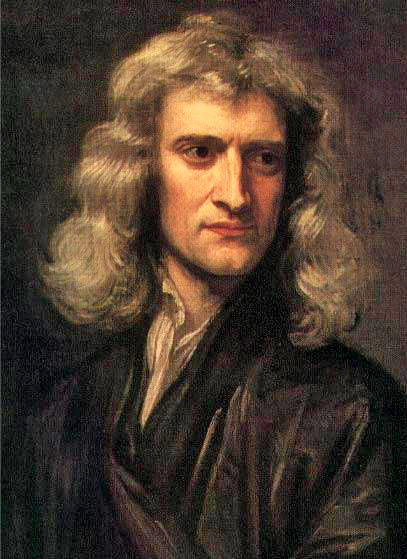
\includegraphics[scale=.25]{newton_portrait.jpg}

\end{multicols}

}

% Section I:
\section{\sectiontitleI}

\frame{
\frametitle{\sectiontitleI}

\textbf{Early Life:}\vspc

Isaac Newton was born (according to the Julian calendar, in use in England at the time) on Christmas Day, 25 December 1642 ... \vspc ... at Woolsthorpe Manor in Woolsthorpe-by-Colsterworth, a hamlet in the county of Lincolnshire. \vspc

{\tiny Text: \href{https://en.wikipedia.org/wiki/Isaac_Newton}{Wikipedia}}
}

\frame{
\frametitle{\sectiontitleI}

\textbf{Education:}\vspc

From the age of about twelve until he was seventeen, Newton was educated at The King's School, Grantham, which taught Latin and Greek and probably  \hspcu\hspcu\hspcu \vspc

In June 1661, he was admitted to Trinity College, Cambridge ... \vspc
... the college's teachings were based on those of Aristotle, whom Newton supplemented with modern philosophers such as Descartes, and astronomers such as Galileo and Thomas Street, through whom he learned of Kepler's work.

{\tiny Text: \href{https://en.wikipedia.org/wiki/Isaac_Newton}{Wikipedia}}
}

\frame{
\frametitle{\sectiontitleI}

\textbf{Development of Calculus:}\vspc

 In 1665, he discovered the generalised binomial theorem and began to develop a mathematical theory that later became calculus. Soon after Newton had obtained his BA degree in August 1665, { \G the university temporarily closed as a precaution against the Great Plague}. Although he had been undistinguished as a Cambridge student,[16] Newton's private studies at his home in Woolsthorpe over the subsequent two years saw the development of his theories on calculus,[17] optics, and the law of gravitation. 

{\tiny Text: \href{https://en.wikipedia.org/wiki/Isaac_Newton}{Wikipedia}}
}

\frame{
\frametitle{\sectiontitleI}

\textbf{Foundation of Mechanics:}\vspc

The Principia was published on 5 July 1687 ... In this work, Newton stated \hspcu\hspcu\hspcu. Together, these laws describe the relationship between any object, the forces acting upon it and the resulting motion, laying {\B the foundation for classical mechanics}. They contributed to many advances during the Industrial Revolution which soon followed and were not improved upon for more than 200 years. Many of these advancements continue to be the underpinnings of non-relativistic technologies in the modern world...

{\tiny Text: \href{https://en.wikipedia.org/wiki/Isaac_Newton}{Wikipedia}}
}

% Section II:
\section{\sectiontitleII}

\frame{
\frametitle{\sectiontitleII}

\textbf{Newton's First Law of Motion}\vspc
{\it Every object persists in its state of rest or uniform motion in a straight line unless it is compelled to change that state by forces impressed on it.}\vspace{30mm}\\



{\tiny Text: \href{https://www.grc.nasa.gov/WWW/K-12/airplane/newton.html}{NASA}}
}

% Section III:
\section{\sectiontitleIII}

\frame{
\frametitle{\sectiontitleIII}

\textbf{Newton's Second Law of Motion}\vspc

{\it Force is equal to the change in momentum ($mV$) per change in time. For a constant mass, force equals mass time acceleration ($F=ma$).}\vspace{30mm}\\



{\tiny Text: \href{https://www.grc.nasa.gov/WWW/K-12/airplane/newton.html}{NASA}}
}

% Section IV:
\section{\sectiontitleIV}

\frame{
\frametitle{\sectiontitleIV}

\textbf{Newton's Third Law of Motion}\vspc

{\it For every action, there is an equal and opposite re-action.}\vspace{30mm}\\



{\tiny Text: \href{https://www.grc.nasa.gov/WWW/K-12/airplane/newton.html}{NASA}}
}
	
\end{document}





